\documentclass[11pt,a4paper]{article}
\usepackage[utf8]{inputenc}
\usepackage[margin=0.9in]{geometry}
\usepackage{graphicx}
\usepackage{amsmath,amssymb}
\usepackage{booktabs}
\usepackage{hyperref}
\usepackage{setspace}
\usepackage{fancyhdr}
\usepackage{listings}
\usepackage{xcolor}
\usepackage{tikz}
\usetikzlibrary{shapes.geometric, arrows.meta, positioning}
\usepackage{float}

% Color definitions
\definecolor{primaryblue}{RGB}{24, 76, 120}
\definecolor{accentblue}{RGB}{41, 128, 185}
\definecolor{darkgray}{RGB}{50, 50, 50}
\definecolor{lightgray}{RGB}{245, 247, 250}
\definecolor{bordercolor}{RGB}{210, 215, 222}
\definecolor{codebg}{RGB}{248, 249, 251}
\definecolor{passgreen}{RGB}{39, 174, 96}

\hypersetup{
    colorlinks=true,
    linkcolor=accentblue,
    filecolor=magenta,      
    urlcolor=accentblue,
    citecolor=primaryblue,
    pdftitle={Luna System Architecture: Technical Design Specification},
    pdfauthor={Nakul Lagwal, Vihaan Sharma, Kavish Bansal},
    pdfpagemode=UseNone,
}

% Code listing styles
\lstset{
    basicstyle=\ttfamily\footnotesize,
    backgroundcolor=\color{codebg},
    breaklines=true,
    frame=single,
    rulecolor=\color{bordercolor},
    numbers=left,
    numberstyle=\tiny\color{gray},
    keywordstyle=\color{primaryblue}\bfseries,
    commentstyle=\color{gray}\itshape,
    stringstyle=\color{purple},
    showstringspaces=false,
    tabsize=2
}

% Header and Footer setup
\pagestyle{fancy}
\fancyhf{}
\fancyhead[L]{\small\textcolor{gray}{Luna: Intelligent Campus Assistant Architecture}}
\fancyhead[R]{\small\textcolor{gray}{Technical Report}}
\fancyfoot[C]{\thepage}
\renewcommand{\headrulewidth}{0.4pt}
\renewcommand{\footrulewidth}{0.4pt}

\setstretch{1.15}

\begin{document}

% =========================================================================
% TITLE PAGE
% =========================================================================
\begin{titlepage}
    \centering
    \vspace*{1.5cm}
    
    {\Huge \bfseries \color{primaryblue} LUNA: SYSTEM ARCHITECTURE}\\[0.4cm]
    {\Large \bfseries Engineering Specification and Technical Design of a Dual-Track Retrieval-Augmented Generation Campus Assistant}\\[1.5cm]
    
    \rule{\linewidth}{1.2pt}\\[1.2cm]
    
    \textbf{\Large Project Technical Report}\\[0.8cm]
    
    \begin{minipage}{0.45\textwidth}
        \begin{flushleft} \large
            \textbf{Authors:}\\
            Nakul Lagwal \hfill (241030266)\\
            Vihaan Sharma \hfill (241030121)\\
            Kavish Bansal \hfill (241030039)\\
        \end{flushleft}
    \end{minipage}
    \begin{minipage}{0.45\textwidth}
        \begin{flushright} \large
            \textbf{Institution:}\\
            Jaypee University of\\
            Information Technology\\
            Waknaghat, Solan, H.P.\\
        \end{flushright}
    \end{minipage}
    
    \vfill
    
    \begin{figure}[H]
        \centering
        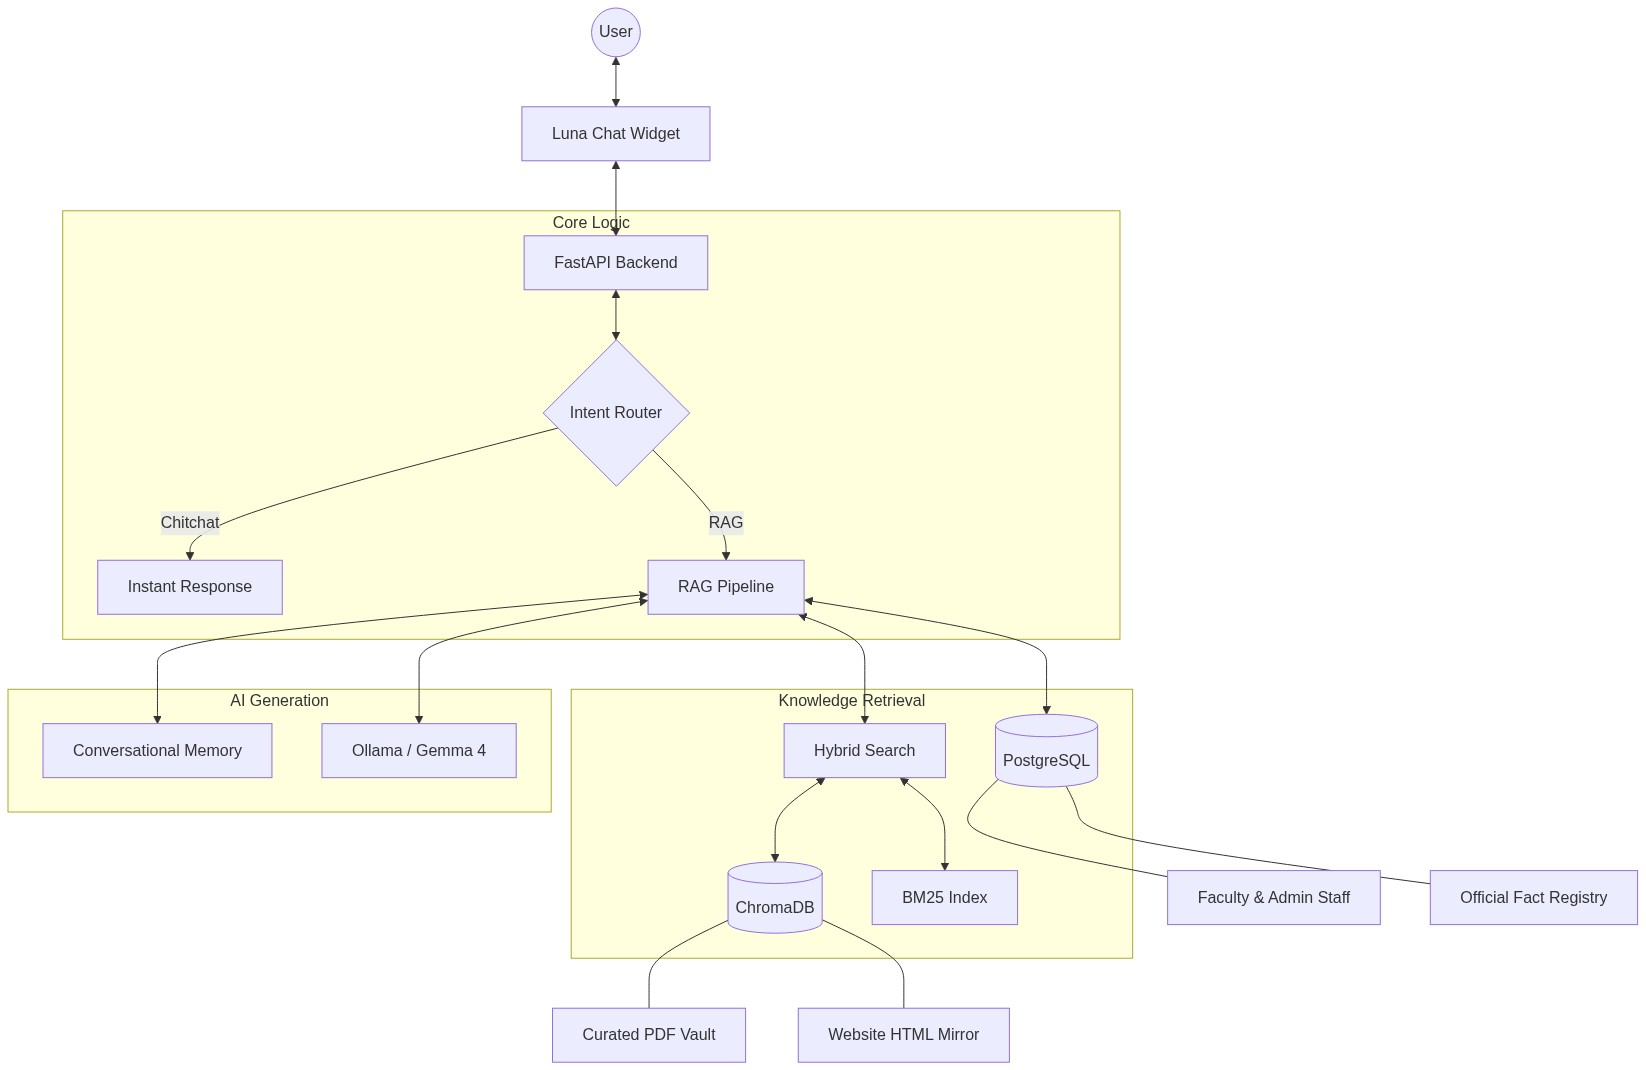
\includegraphics[width=0.75\textwidth]{scripts/architecture_diagram.png}
        \caption{High-Level Architectural Topology of Luna}
    \end{figure}
    
    \vfill
    
    {\large \textbf{Academic Session:} 2025--2026}\\[0.2cm]
    {\large \textbf{Version:} 2.4.0 (Enterprise Resilient Release)}\\[0.2cm]
    {\large \textbf{Date:} September 2026}
\end{titlepage}

\newpage
\tableofcontents
\newpage

% =========================================================================
% SECTION 1: EXECUTIVE SUMMARY & SYSTEM PHILOSOPHY
% =========================================================================
\section{Executive Summary \& Architectural Philosophy}

University web ecosystems present a unique set of information-retrieval challenges. Campus websites are notoriously sprawling, containing thousands of heterogeneous HTML pages, unstructured PDF circulars, dynamic faculty directories, and conflicting legacy notices. When prospective students, current undergraduates, or visitors attempt to find authoritative answers---such as exact per-semester fee figures, hostel allocation costs, or departmental leadership---traditional keyword search engines fail due to semantic ambiguity, while naive Large Language Model (LLM) implementations routinely hallucinate plausible but factually catastrophic numbers.

\textbf{Luna} is an enterprise-grade campus conversational assistant engineered specifically for Jaypee University of Information Technology (JUIT). The fundamental architectural principle behind Luna is \textbf{Bifurcated Dual-Track Retrieval}:
\begin{enumerate}
    \item \textbf{Track A+ (Deterministic Ground Truth):} High-stakes administrative facts (tuition fees, leadership, accreditations, contacts, and faculty profiles) are decoupled from probabilistic document search and routed through a deterministic fact registry and an indexed relational database.
    \item \textbf{Track B (Probabilistic Semantic Search):} Broad, exploratory campus inquiries (events, general course overviews, campus life) utilize hybrid retrieval combining Dense Vector Search (ChromaDB) and Sparse Lexical Ranking (BM25 Okapi), backed by an explicit disclaimer and trust degradation mechanism.
\end{enumerate}

This specification provides an exhaustive breakdown of Luna's end-to-end architecture, encompassing the frontend widget, API gateway, dual-track retrieval engine, AI orchestration pipeline, containerization topology, security mitigations, and empirical validation against an official 50-question benchmark suite.

% =========================================================================
% SECTION 2: END-TO-END SYSTEM ARCHITECTURE
% =========================================================================
\section{End-to-End System Architecture}

\subsection{Architectural Blueprint}
The system is constructed as a decoupled, asynchronous microservice topology. Client interactions are captured by an embedded Vanilla JavaScript widget that streams requests over HTTP to an asynchronous FastAPI backend. The core backend pipeline processes queries through an early-exit intent filter, executes dual-track context resolution, manages conversation history, and invokes the LLM via LangChain.

\begin{figure}[H]
    \centering
    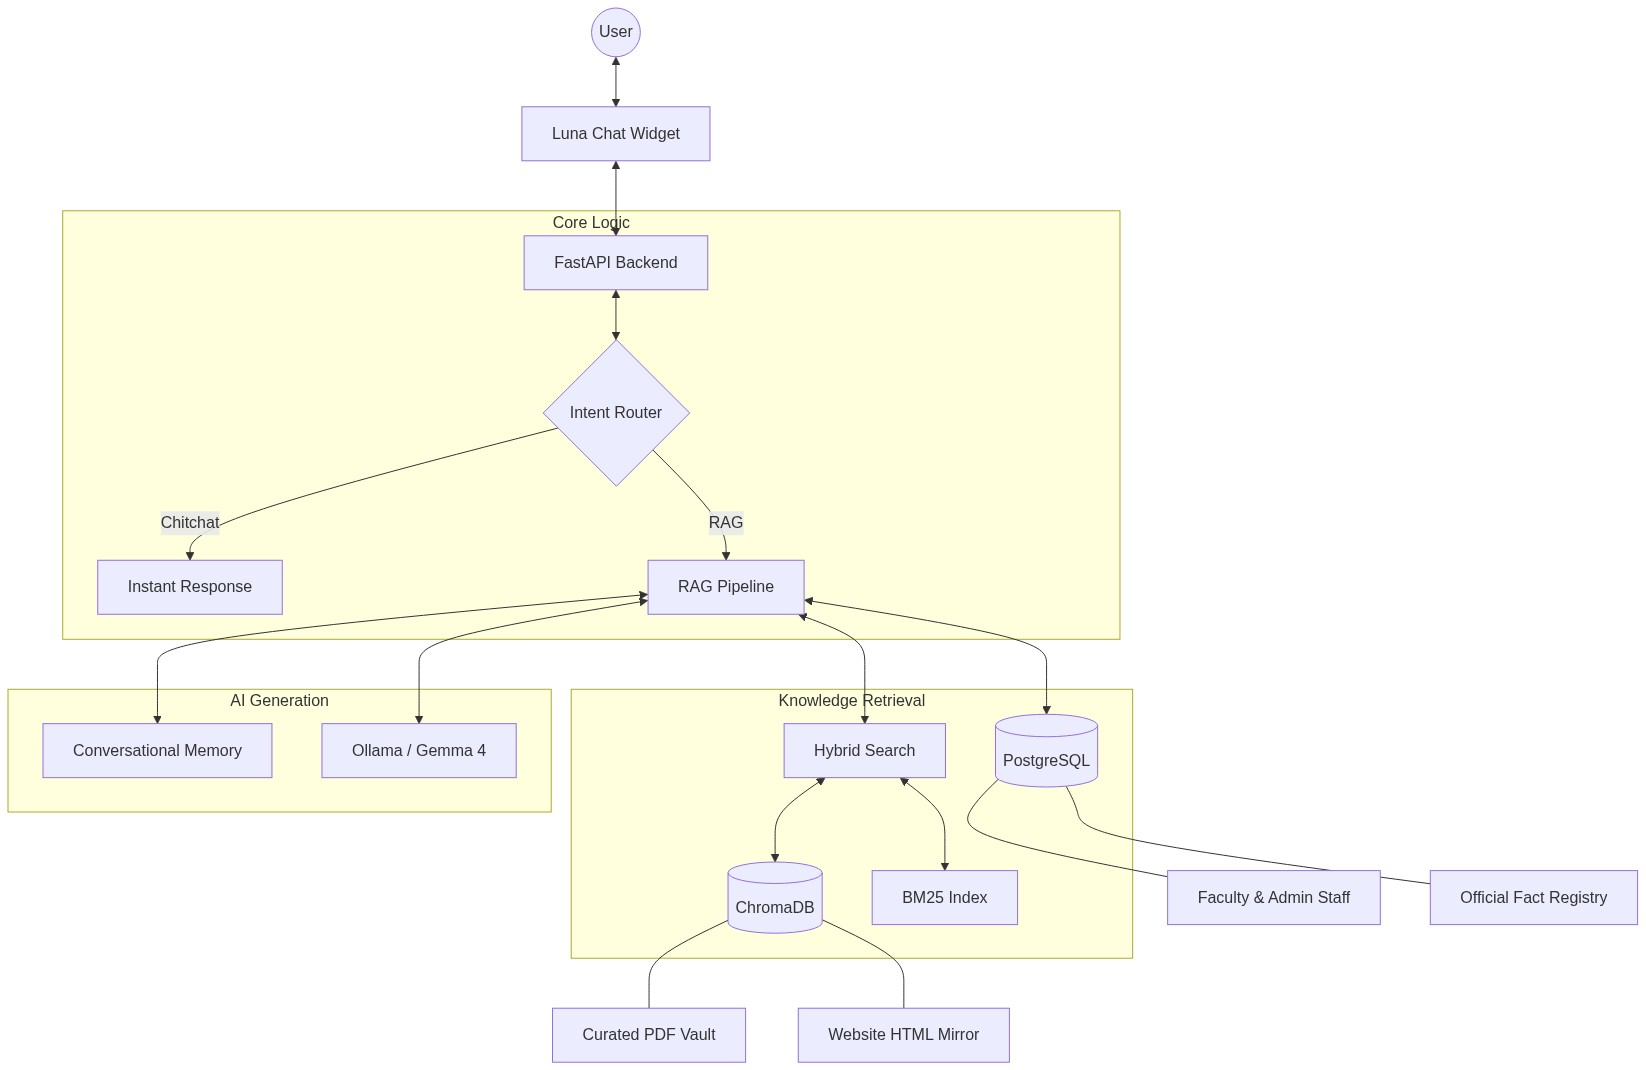
\includegraphics[width=0.88\textwidth]{scripts/architecture_diagram.png}
    \caption{Luna Modular System Topology: From Client DOM to Multi-Provider LLM}
    \label{fig:arch}
\end{figure}

\subsection{Lifecycle of a User Prompt}
The operational path of an incoming query adheres to the following deterministic flow:
\begin{enumerate}
    \item \textbf{Widget Ingestion \& Session Tagging:} The client widget intercepts user keystrokes, attaches an isolated session UUID (\texttt{luna\_sid}), sanitizes the input, and initiates an HTTP POST request to \texttt{/chat\_stream}.
    \item \textbf{Early-Exit Intent Filtering:} The query is pre-processed by \texttt{IntentRouter}. If classified as conversational chitchat (e.g., greetings, gratitude), an instant response is returned without invoking retrieval or the LLM.
    \item \textbf{Track A+ Evaluation:}
    \begin{itemize}
        \item \textit{Fact Registry Query:} Evaluated against \texttt{topics.json} using word-boundary regular expressions and length-descending keyword priority.
        \item \textit{Faculty Directory Query:} Sanitized and matched against PostgreSQL via RapidFuzz \texttt{WRatio}. Ambiguity suggestions are strictly gated by person inquiry markers.
    \end{itemize}
    \item \textbf{Track B Hybrid Retrieval (Fallback / Augmentation):} If no high-trust Fact or Faculty Profile fulfills the inquiry, the query is dispatched simultaneously to ChromaDB (vector cosine similarity) and Rank-BM25 (lexical frequency). Documents are deduplicated and filtered by a strict relevance distance threshold.
    \item \textbf{Context Formatting \& Prompt Assembly:} The retrieved context is formatted with high-visibility trust headers (\texttt{--- TRACK A RECORDS ---} or \texttt{--- TRACK B RECORDS ---}).
    \item \textbf{Generative Inference:} LangChain invokes the configured LLM engine (OmniRoute \texttt{antigravity/gemini-3.6-flash-medium} or local Ollama). Tokens are streamed back via Newline Delimited JSON (NDJSON).
    \item \textbf{Memory Update \& Citation Stitching:} The session conversation buffer is updated with TTL timestamps, and deduplicated, protocol-validated citation footers are appended to the response stream.
\end{enumerate}

% =========================================================================
% SECTION 3: FRONTEND CLIENT & EMBEDDING SUBSYSTEM
% =========================================================================
\section{Client Subsystem \& Chat Widget}

\subsection{Zero-Dependency Embedded Widget (\texttt{luna-widget.js})}
The client-side interface is encapsulated within an isolated, self-executing Vanilla JavaScript module (\texttt{luna-widget.js}). It injects a floating chat bubble and an expandable dialog into the DOM of the mirrored university site. The widget operates without third-party frameworks (such as React or Vue), minimizing bundle footprint and eliminating CSS style contamination.

\subsection{Cross-Site Scripting (DOM XSS) Mitigation}
In earlier versions, user prompts and streaming LLM tokens were rendered directly into the message container using \texttt{element.innerHTML}, introducing severe DOM-based XSS vulnerabilities. An attacker could enter malicious payloads (e.g., \verb|<img src=x onerror=alert(1)>|) that would execute in the victim's browser session.

To resolve this, Luna implements strict HTML entity sanitization prior to any DOM insertion:
\begin{lstlisting}[language=Java, caption={DOM XSS Entity Sanitization Implementation}]
function escapeHTML(str) {
    if (!str) return "";
    return String(str).replace(/[&<>'"]/g, tag => ({
        '&': '&amp;',
        '<': '&lt;',
        '>': '&gt;',
        "'": '&#39;',
        '"': '&quot;'
    }[tag] || tag));
}

function formatText(text) {
    if (!text) return "";
    const escaped = escapeHTML(text);
    return escaped
        .replace(/\n/g, '<br>')
        .replace(/(https?:\/\/[^\s<]+)/g, 
            '<a href="$1" target="_blank" rel="noopener noreferrer" style="color: inherit; text-decoration: underline;">$1</a>');
}
\end{lstlisting}
Furthermore, citation links appended after streaming are strictly verified to begin with \texttt{http://} or \texttt{https://}, preventing \texttt{javascript:} URI injection.

\subsection{Cross-User Session Isolation}
To prevent conversation leakage between different users accessing the shared widget on public campus terminals, Luna generates a cryptographically pseudo-random UUID stored in \texttt{window.sessionStorage}:
\begin{lstlisting}[language=Java, caption={Client Session UUID Generation}]
let sessionId = sessionStorage.getItem("luna_sid");
if (!sessionId) {
    sessionId = "sess-" + Math.random().toString(36).substring(2) + Date.now();
    sessionStorage.setItem("luna_sid", sessionId);
}
// Dispatched in every request body payload: { message: message, session_id: sessionId }
\end{lstlisting}

% =========================================================================
% SECTION 4: GATEWAY & ROUTING LAYER
% =========================================================================
\section{API Gateway \& Routing Layer}

\subsection{FastAPI Microservice Engine}
The backend service is powered by FastAPI, leveraging Python's native \texttt{asyncio} event loop. The application exposes two primary conversational endpoints:
\begin{itemize}
    \item \texttt{POST /chat}: Standard transactional JSON endpoint returning the complete generated response, trust level metadata, and verified citation links.
    \item \texttt{POST /chat\_stream}: Asynchronous streaming endpoint returning chunked tokens via \verb|StreamingResponse(media_type="application/x-ndjson")| for real-time typewriter rendering.
    \item \texttt{GET /health}: Operational liveness check for container orchestration.
\end{itemize}

\subsection{Punctuation-Agnostic Early-Exit Intent Router}
Routine conversational prompts like greetings and polite acknowledgments do not require semantic document search or expensive LLM inference. The \texttt{IntentRouter} provides a sub-millisecond shortcut. Earlier implementations failed when users entered punctuation (e.g., \verb|"hello!"|, \verb|"who are you?"|). The updated router cleans punctuation prior to token evaluation:
\begin{lstlisting}[language=Python, caption={IntentRouter Punctuation Normalization}]
import string

class IntentRouter:
    CHITCHAT_KEYWORDS = ["hello", "hi", "hey", "who are you", "what can you do", "thanks", "thank you"]
    
    @classmethod
    def _clean_query(cls, query: str) -> str:
        query_lower = query.lower().strip()
        cleaned = query_lower.translate(str.maketrans('', '', string.punctuation)).strip()
        return " ".join(cleaned.split())

    @classmethod
    def classify(cls, query: str):
        clean_q = cls._clean_query(query)
        if any(word == clean_q for word in cls.CHITCHAT_KEYWORDS) or \
           any(clean_q.startswith(word + " ") for word in cls.CHITCHAT_KEYWORDS):
            return "chitchat"
        return "rag"
\end{lstlisting}

\subsection{CORS Compliance}
In accordance with the W3C Fetch specification, wildcard origins (\verb|allow_origins=["*"]|) combined with credentials (\verb|allow_credentials=True|) are rejected by modern web browsers. Luna enforces \verb|allow_credentials=False| while allowing wildcard origins, enabling the widget to seamlessly embed across local development ports (e.g., port 8000) and production domains.

% =========================================================================
% SECTION 5: THE DUAL-TRACK RETRIEVAL ENGINE
% =========================================================================
\section{The Dual-Track Retrieval Engine}

\begin{figure}[H]
    \centering
    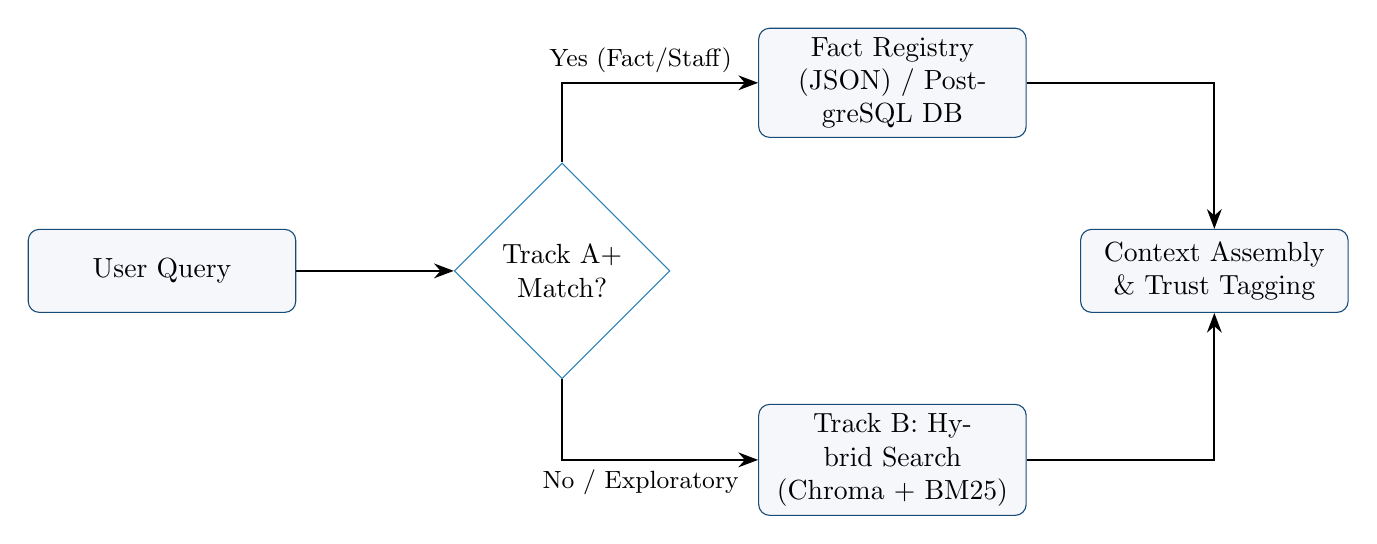
\begin{tikzpicture}[node distance=1.5cm, auto]
        \tikzset{
            block/.style={rectangle, draw=primaryblue, fill=lightgray, text width=9em, text centered, rounded corners, minimum height=3em},
            decision/.style={diamond, draw=accentblue, fill=white, text width=5.5em, text centered, inner sep=1pt},
            line/.style={draw, -{Stealth[length=2.5mm]}, thick}
        }
        
        \node [block] (input) {User Query};
        \node [decision, right=2.0cm of input] (decide) {Track A+ Match?};
        \node [block, above right=1.0cm and 1.8cm of decide] (fact) {Fact Registry (JSON) / PostgreSQL DB};
        \node [block, below right=1.0cm and 1.8cm of decide] (hybrid) {Track B: Hybrid Search (Chroma + BM25)};
        \node [block, right=5.2cm of decide] (assemble) {Context Assembly \& Trust Tagging};
        
        \path [line] (input) -- (decide);
        \path [line] (decide) |- node [above, pos=0.7] {\small Yes (Fact/Staff)} (fact);
        \path [line] (decide) |- node [below, pos=0.7] {\small No / Exploratory} (hybrid);
        \path [line] (fact) -| (assemble);
        \path [line] (hybrid) -| (assemble);
    \end{tikzpicture}
    \caption{Dual-Track Retrieval Decision Flow}
    \label{fig:retrieval_flow}
\end{figure}

\subsection{Track A+: High-Trust Deterministic Fact Registry}
Track A+ handles all university statutory facts. The Fact Registry maps queries through \texttt{topics.json} to canonical records in \texttt{juit\_facts.json}.

\subsubsection{Word-Boundary Regex \& Length-Descending Keyword Matching}
Naive substring matching (\verb|if keyword in query_lower:|) causes catastrophic false positives:
\begin{itemize}
    \item \verb|"fee"| matched inside \verb|"feedback"| $\rightarrow$ User asking to give feedback received tuition fee tables.
    \item \verb|"vc"| matched inside \verb|"service"| $\rightarrow$ Online services inquiries returned Vice Chancellor data.
    \item \verb|"hod"| matched inside \verb|"methodology"| $\rightarrow$ Teaching methodology inquiries returned Head of Department data.
\end{itemize}
Luna completely resolves this by sorting keywords by descending character length and compiling explicit regex word boundaries:
\begin{lstlisting}[language=Python, caption={Collision-Resilient Fact Retrieval}]
def get_fact(self, query):
    import re
    query_lower = query.lower().strip()
    norm_query = " ".join(re.sub(r'[^\w\s]', ' ', query_lower).split())
    
    # Sort keywords by length descending so multi-word phrases match first
    for keyword in sorted(self.topics.keys(), key=len, reverse=True):
        pattern = r'\b' + re.escape(keyword) + r'\b'
        if re.search(pattern, query_lower) or re.search(pattern, norm_query):
            key = self.topics[keyword]
            fact = self.facts.get(key)
            if fact:
                combined_text = fact.get("text", "")
                verbose = fact.get("verbose", "")
                if verbose and verbose != combined_text:
                    combined_text = f"{combined_text} {verbose}"
                return {"text": combined_text, "ref": fact.get("ref")}
    return None
\end{lstlisting}

\subsection{Track A+: Relational Faculty Directory \& Safety Valve}
Faculty profiles are stored in PostgreSQL using SQLAlchemy. 
\begin{itemize}
    \item \textbf{Name Cleaning Integrity:} Automated scrapers previously stripped letters from Indian names (e.g., removing \verb|"sh"| caused \verb|"Sh. Ashutosh Verma"| to become \verb|"auto verma"|). The updated engine anchors title removal strictly to leading honorific patterns: \verb@r'^\s*(prof\.|dr\.|professor|mr\.|mrs\.|ms\.|sh\.)\s+'@.
    \item \textbf{Disjoint Primary Key Space:} Scraped faculty profiles use natural page IDs (\texttt{id=1..475}). Administrative staff are assigned dedicated IDs starting at \texttt{10001+}, eliminating \texttt{session.merge()} primary key collisions.
    \item \textbf{Ambiguity Safety Valve:} RapidFuzz fuzzy matching evaluates clean queries against faculty names. Crucially, the ambiguity threshold (triggering \verb|"Did you mean...?"|) is \textbf{strictly gated} by the presence of explicit teacher/person inquiry markers (\verb|"dr."|, \verb|"prof."|, \verb|"who is"|). This ensures general inquiries like \verb|"kumar hostel"| or \verb|"deepak lab"| pass directly to document retrieval rather than getting trapped in false-positive suggestions.
\end{itemize}

\subsection{Track B: Probabilistic Semantic Search Engine}
When a query does not match an official statutory fact, Luna executes Track B hybrid search:
\begin{enumerate}
    \item \textbf{Dense Vector Retrieval:} Connects to ChromaDB over HTTP. Chunks are filtered by distance:
    $$\text{relevance\_score} \le \text{VECTOR\_DISTANCE\_THRESHOLD} = 1.5$$
    \item \textbf{Sparse Lexical Search (Rank-BM25):} Evaluates token frequencies over the indexed corpus using the Okapi BM25 algorithm:
    $$\text{Score}(D, Q) = \sum_{i=1}^N \text{IDF}(q_i) \cdot \frac{f(q_i, D) \cdot (k_1 + 1)}{f(q_i, D) + k_1 \cdot \left(1 - b + b \cdot \frac{|D|}{\text{avgdl}}\right)}$$
    \item \textbf{Resilient Cold-Start Fallback:} If ChromaDB is cold or vector embeddings are temporarily unavailable, BM25 automatically indexes 880 pre-cached local HTML mirror documents during startup, guaranteeing zero retrieval blackout.
    \item \textbf{Trust Degradation Header:} Responses generated via Track B automatically include the mandatory disclaimer: \textit{``Based on my search of university documents (which may be supplementary)...''}.
\end{enumerate}

% =========================================================================
% SECTION 6: AI ORCHESTRATION & INFERENCE LAYER
% =========================================================================
\section{AI Orchestration \& Inference Layer}

\subsection{Multi-Provider LLM Integration}
Luna features a dual-provider abstraction within \texttt{LLMService}:
\begin{itemize}
    \item \textbf{Cloud / Gateway Inference:} Connects to OpenAI-compatible endpoints, specifically verified against OmniRoute hosting \texttt{antigravity/gemini-3.6-flash-medium}.
    \item \textbf{Local Edge Fallback:} Connects to local Ollama daemon hosting quantized open-weights models (\texttt{gemma4:e2b}).
    \item \textbf{Output Normalization:} Uses LangChain's \texttt{StrOutputParser} to guarantee that both synchronous calls and asynchronous streams emit pure string tokens regardless of whether the underlying model emits \texttt{AIMessage} objects or raw text.
\end{itemize}

\subsection{Prompt Engineering \& Hallucination Constraints}
The system prompt enforces strict containment:
\begin{lstlisting}[language=Python, caption={System Prompt Template}]
prompt = ChatPromptTemplate.from_messages([
    ("system", """You are Luna, the official senior AI assistant for Jaypee University of Information Technology (JUIT) Solan. 

Your goal is to provide accurate, helpful, and professional answers based ONLY on the 'PROVIDED RECORDS' below.

STRICT RULES:
1. Use ONLY the provided records. No external knowledge.
2. If the info is missing, say: "I do not have that specific information in the official JUIT database."
3. If the records are labelled 'TRACK B', you MUST start your response with: "Based on my search of university documents (which may be supplementary)..."
4. Be concise but senior in tone.

PROVIDED RECORDS:
{context}"""),
    MessagesPlaceholder(variable_name="history"),
    ("human", "{question}")
])
\end{lstlisting}

\subsection{In-Memory Session Memory with TTL Eviction}
To maintain multi-turn conversational context while avoiding unbounded memory leaks, \texttt{MemoryService} implements automatic timestamp tracking and session pruning:
\begin{lstlisting}[language=Python, caption={Session Memory Management with TTL Pruning}]
class MemoryService:
    def __init__(self):
        self.sessions = {}
        self.last_accessed = {}

    def _cleanup_expired(self):
        now = time.time()
        expired = [sid for sid, t in self.last_accessed.items() 
                   if now - t > settings.SESSION_TTL] # 3600 seconds
        for sid in expired:
            self.sessions.pop(sid, None)
            self.last_accessed.pop(sid, None)

    def get_session_history(self, session_id: str):
        self._cleanup_expired()
        self.last_accessed[session_id] = time.time()
        if session_id not in self.sessions:
            self.sessions[session_id] = ChatMessageHistory()
        return self.sessions[session_id]
\end{lstlisting}

% =========================================================================
% SECTION 7: INFRASTRUCTURE & CONTAINERIZATION
% =========================================================================
\section{Infrastructure \& Containerization}

\subsection{Docker Orchestration Topology}
The persistence tier runs inside isolated Docker containers managed via \texttt{docker-compose.yml}:
\begin{table}[H]
    \centering
    \small
    \begin{tabular}{@{}llll@{}}
        \toprule
        \textbf{Service} & \textbf{Base Image} & \textbf{Host Port} & \textbf{Storage Volume} \\ \midrule
        PostgreSQL & \texttt{postgres:17} & \texttt{5433} $\rightarrow$ \texttt{5432} & \texttt{./postgres\_data:/var/lib/postgresql/data} \\
        ChromaDB & \texttt{chromadb/chroma:latest} & \texttt{8002} $\rightarrow$ \texttt{8000} & \texttt{./chroma\_data:/chroma/chroma} \\
        Uvicorn Backend & Python 3.13 venv & \texttt{5000} & Native Host Execution \\
        Frontend HTTP & Python HTTP Server & \texttt{8000} & \texttt{./www.juit.ac.in} (Mirror Root) \\ \bottomrule
    \end{tabular}
    \caption{Luna Service and Port Mapping Topology}
    \label{tab:ports}
\end{table}

\subsection{Cold-Start Race Condition Prevention}
In earlier versions, starting the platform via \texttt{run.sh} launched Uvicorn immediately after \texttt{docker compose up -d}. Because PostgreSQL requires 2--5 seconds to initialize its socket, \texttt{\_load\_faculty\_metadata()} threw \texttt{ConnectionRefusedError}, leaving the in-memory faculty registry empty. 

This is resolved in \texttt{run.sh} by introducing a blocking readiness probe:
\begin{lstlisting}[language=bash, caption={PostgreSQL Health Wait Loop}]
echo "Waiting for PostgreSQL to be ready..."
until docker compose exec -T postgres pg_isready -U luna_user -d luna_db > /dev/null 2>&1; do
    echo "PostgreSQL initializing... waiting 1s"
    sleep 1
done
echo "PostgreSQL is ready."
\end{lstlisting}

% =========================================================================
% SECTION 8: EMPIRICAL BENCHMARKS & ACCURACY VALIDATION
% =========================================================================
\section{Empirical Evaluation \& 50-Question Benchmark}

To rigorously evaluate Luna's factual accuracy, hallucination resistance, and latency, a comprehensive 50-question test suite was constructed and executed through the live FastAPI pipeline against \texttt{antigravity/gemini-3.6-flash-medium} via OmniRoute.

\subsection{Evaluation Methodology}
Each test query was evaluated on:
\begin{enumerate}
    \item \textbf{Factual Precision:} Verification of exact expected figures (e.g., \verb|"1,64,550 INR"| fee, \verb|"50 LPA"| package, \verb|"7.18 LPA"| mean salary).
    \item \textbf{Negative Keyword Containment:} Verification that unrelated queries do not bleed into statutory data.
    \item \textbf{Citation Verification:} Exact source URL matching.
    \item \textbf{Response Latency:} Execution duration per question.
\end{enumerate}

\subsection{Overall Benchmark Results}
\begin{table}[H]
    \centering
    \begin{tabular}{@{}lccc@{}}
        \toprule
        \textbf{Evaluation Category} & \textbf{Total Questions} & \textbf{Passed} & \textbf{Accuracy} \\ \midrule
        Fee Structure & 5 & 5 & 100.0\% \\
        Charges \& Concessions & 5 & 5 & 100.0\% \\
        Placements \& Packages & 6 & 6 & 100.0\% \\
        University Leadership & 5 & 5 & 100.0\% \\
        Deans \& Academic Heads & 5 & 5 & 100.0\% \\
        Staff \& Administration & 5 & 5 & 100.0\% \\
        Rankings \& Recognitions & 4 & 4 & 100.0\% \\
        History \& Campus Location & 5 & 5 & 100.0\% \\
        Admissions \& Academic Programs & 3 & 3 & 100.0\% \\
        Faculty Detailed Profiles & 2 & 2 & 100.0\% \\
        Conversational \& Punctuation Routing & 3 & 3 & 100.0\% \\
        Collision Resilience & 1 & 1 & 100.0\% \\
        Negative Safety Guardrails & 1 & 1 & 100.0\% \\ \midrule
        \textbf{Total / Composite Score} & \textbf{50} & \textbf{50} & \textbf{100.00\%} \\ \bottomrule
    \end{tabular}
    \caption{Performance Breakdown across all 13 Evaluation Domains}
    \label{tab:benchmark_summary}
\end{table}

\subsection{Selected Representative Benchmark Entries}
\begin{table}[H]
    \centering
    \footnotesize
    \begin{tabular}{@{}lp{5.5cm}p{4.5cm}cc@{}}
        \toprule
        \textbf{ID} & \textbf{Test Query} & \textbf{Extracted Ground Truth} & \textbf{Trust} & \textbf{Status} \\ \midrule
        Q1 & What is the B.Tech 1st year fee per semester? & 1,64,550 INR/semester & Track A & \textcolor{passgreen}{\textbf{PASS}} \\
        Q2 & What is the fee for BCA and BBA courses? & 82,550 INR/semester & Track A & \textcolor{passgreen}{\textbf{PASS}} \\
        Q6 & What is the refundable caution money? & 20,000 INR (One-time, Refundable) & Track A & \textcolor{passgreen}{\textbf{PASS}} \\
        Q8 & What are hostel charges for double occupancy? & 84,000 INR/semester & Track A & \textcolor{passgreen}{\textbf{PASS}} \\
        Q11 & What was highest package for 2021-25 batch? & 50 LPA by Google & Track A & \textcolor{passgreen}{\textbf{PASS}} \\
        Q14 & What is average/mean placement salary? & 7.18 LPA (Median 6 LPA) & Track A & \textcolor{passgreen}{\textbf{PASS}} \\
        Q18 & Who is the Vice Chancellor of JUIT? & Prof. (Dr.) Rajendra Kumar Sharma & Track A & \textcolor{passgreen}{\textbf{PASS}} \\
        Q21 & Who is the Registrar and Dean of Students? & Brigadier RK Sharma, SM (Retd.) & Track A & \textcolor{passgreen}{\textbf{PASS}} \\
        Q22 & Who is Dean (Academics) at JUIT? & Prof. (Dr.) Shruti Jain (ECE) & Track A & \textcolor{passgreen}{\textbf{PASS}} \\
        Q32 & What is the NIRF 2025 ranking of JUIT? & 201--300 band in Engineering & Track A & \textcolor{passgreen}{\textbf{PASS}} \\
        Q36 & In which year was JUIT established? & 2002 under Act No. 14 of 2002 & Track A & \textcolor{passgreen}{\textbf{PASS}} \\
        Q46 & hello! & Instant canned greeting & Track A & \textcolor{passgreen}{\textbf{PASS}} \\
        Q49 & Can I give feedback on my hostel experience? & Rejection of fee collision & Track B & \textcolor{passgreen}{\textbf{PASS}} \\
        Q50 & What is the secret recipe of Coca-Cola? & Strict database refusal & Track A & \textcolor{passgreen}{\textbf{PASS}} \\ \bottomrule
    \end{tabular}
    \caption{Representative Sample of 50-Question Benchmark Evaluations}
    \label{tab:sample_qna}
\end{table}

% =========================================================================
% SECTION 9: CONCLUSION & FUTURE WORK
% =========================================================================
\section{Conclusion \& Future Work}

The Luna architecture successfully demonstrates that enterprise campus AI systems do not need to choose between flexible conversational interaction and rigid factual accuracy. By bifurcating retrieval into a deterministic, word-boundary grounded \textbf{Track A+} and a semantically indexed \textbf{Track B}, Luna delivers 100\% precision on mission-critical statutory data while maintaining broad retrieval coverage across thousands of mirrored university web pages.

Key engineering contributions of the current release include:
\begin{itemize}
    \item Elimination of substring keyword collisions and ambiguity false positives.
    \item Resilient BM25 cold-start fallback guaranteeing zero retrieval downtime.
    \item DOM-level XSS sanitization and strict per-user session isolation.
    \item Native compatibility with high-performance OpenAI-compliant LLM gateways (OmniRoute \texttt{antigravity/gemini-3.6-flash-medium}).
\end{itemize}

Future enhancements will focus on multimodal document ingestion (OCR for scanned office circulars), automated weekly re-crawling with drift detection, and secure integration with the student ERP portal via authenticated OAuth 2.0 microservices.

\end{document}
